\documentclass[final, letterpaper, square, comma, numbers, sort&compress]{elsarticle}
\usepackage[utf8]{inputenc}
\usepackage[
    % margin=1in
    top=1in,
    bottom=0.7in,
    left=1in,
    right=1in,
    %footskip=0.5in, % FIXME: temp fix
    footnotesep=0.3in,
    % showframe % Uncomment to show frames around the margins for debugging purposes
]{geometry}

\usepackage{hyperref}
\hypersetup{
	% colorlinks=true, % Whether to color the text of links
	% urlcolor=black, % Color for \url and \href links
	% linkcolor=black, % Color for \nameref links
	% citecolor=black, % Color of reference citations
        hidelinks,
        pdfauthor={R. Ranjan; J. Wilson; M. Barisik; V. Ramanuj; R. Sankaran;},
        pdftitle={Effects of Operating Conditions on the Gas-Phase Decomposition of MTS/H2 during Chemical Vapor Infiltration of SiC} % these lines are nessesary to avoid hyperref throwing errors from pulling the newline in the given frontmatter title section
}

\usepackage{graphicx}
\graphicspath{{figures/}}
\usepackage{amssymb}
\usepackage{amsmath}
\usepackage{array}
\usepackage[bottom]{footmisc}

\journal{Energy Policy} % FIXME

\begin{document}

\begin{frontmatter}


%% Title, authors and addresses
\title{Effects of Operating Conditions on the Gas-Phase Decomposition of \\ MTS/H$_2$ during Chemical Vapor Infiltration of SiC }

\author[1]{R.~Ranjan\corref{cor1}}
\ead{reetesh-ranjan@utc.edu}
\author[1]{J.~Wilson}
\author[1]{M.~Barisik}
\author[2]{V.~Ramanuj}
\author[2]{R.~Sankaran}
\cortext[cor1]{Corresponding author}

\address[1]{Department of Mechanical Engineering, The University of Tennessee Chattanooga \\
615 McCallie Avenue, Chattanooga, TN 37403, USA}
\address[2]{Computational Sciences and Engineering Division, Oak Ridge National Laboratory \\
1 Bethel Valley Rd., Oak Ridge, TN 37831, USA}

\begin{abstract}
The quality of the silicon carbide (SiC) matrix composite, which has excellent thermo-mechanical properties, fabricated by the well-established chemical vapor infiltration (CVI) process, depends upon the gas-phase decomposition of the employed precursor and the subsequent heterogeneous reactions at the deposition surface. The decomposition process is primarily affected by the operating parameters such as temperature, pressure, gradient of pressure and temperature, and the composition of the incoming gas-phase reactants. In this study, we perform plug flow reactor (PFR) analysis to examine the effects of operating parameters on the decomposition of the mixture of methyltrichlorosilane (MTS) and hydrogen ($\rm H_2$), a widely used precursor for the manufacturing of SiC matrix composite using the CVI process. The PFR analysis is performed using three chemical mechanisms of increasing degree of complexity, which include globally reduced (1 step and 5 species), moderately complex (30 steps and 20 species), and detailed (103 steps and 42 species) mechanisms. First, we discuss the reduction strategy to obtain the moderately complex mechanism from the detailed one and assess the performance of the three mechanisms by comparing PFR results at atmospheric pressure with reference experimental and numerical results. Afterward, the PFR analysis is performed using these mechanisms at conditions relevant to CVI. These include a range of temperature (1100 K to 1600 K), pressure (5 Torr to 100 Torr), temperature gradient (-190 K/m to -19 K/m), and pressure gradient (-7.7 Torr/m to -0.97 Torr/m). The analysis of the results pertaining to the decomposition of MTS and production of several intermediate reactive species shows that the decomposition of MTS is more sensitive to temperature and its gradient than pressure or pressure gradient. The effects of the ratio of MTS and H2 in the incoming mixture (0.05 to 0.2) are examined by considering isothermal and temperature-gradient conditions. The results show enhanced decomposition of MTS in the case with the presence of a temperature gradient for the same mixture composition, and a nonlinear dependence of the decomposition of MTS and production of intermediates and byproducts on the incoming mixture composition. The present study also showed that the moderately complex chemical kinetics show good agreement with the detailed mechanism, whereas the globally reduced chemical mechanism yielded inaccurate results, thus implying that the moderately complex mechanism can be used while performing detailed three-dimensional modeling of the CVI process.
\end{abstract}

\begin{keyword}
Chemical vapor infiltration \sep silicon carbide \sep methyltrichlorosilane \sep plug flow reactor \sep chemical mechanisms
\end{keyword}

\end{frontmatter}

\let\thefootnote\relax\footnote{Notice: This manuscript has been authored by UT-Battelle, LLC, under contract DEAC05-00OR22725 with the US Depart-ment of Energy (DOE). The US government retains and the publisher, by accepting the article for publication, acknowledges that the US government retains a nonexclusive, paid-up, irrevocable, worldwide license to publish or reproduce the published form of this manuscript, or allow others to do so, for US government purposes. DOE will provide public access to these results of federally sponsored research in accordance with the DOE Public Access Plan (\ttfamily \href{http://energy.gov/downloads/doe-public-access-plan}{http://energy.gov/downloads/doe-public-access-plan}).}

\section{Introduction}
\label{S:1}

Materials that can withstand high-temperature environments are required in many engineering applica- tions such as nuclear reactors, automotive, spacecraft, aircraft components, furnace linings, power electronics,
and cutting and grinding tools. Such materials include metals and alloys (titanium alloys, tungsten, molyb- denum), ceramics (alumina, silicon carbide (SiC), graphite), and composites (ceramic matrix composites, carbon-carbon composites)~\cite{Meetham1991,Tressler1999,Belmonte2006,Fahrenholtz2014,BarCohen2014}. SiC is one such material, which has excellent properties such as high strength, high thermal conductivity, low thermal expansion, chemical inertness, and good thermal shock strength~\cite{Levinshtein2001,Hironaka2002,Snead2007,Presser2008}. However, it also tends to have a low toughness~\cite{Padture1994,Mulla1994,Cao1995}, which has motivated interest in high purity and high quality SiC fiber-reinforced matrix composites~\cite{Naslain1995,Prewo1989,Besmann1991,Wang1996,Prouhet1994,Zhu1999,Liu2023}. In such composites, a SiC matrix is deposited within a fiber preform composed of high-purity, near-stoichiometric SiC fiber. Such an approach leads to a better fracture toughness property while still having a similar performance under high thermal- loading conditions. The deposition of the SiC matrix composites depends upon the operating conditions, which affect the gas-phase decomposition and the subsequent heterogeneous surface reactions on the fiber preform. The present study examines the effects of operating conditions on the gas-phase decomposition of the precursor and the production of intermediate reactive species during SiC matrix deposition.


SiC matrix composites can be fabricated using approaches such as melt infiltration~\cite{Xu1999,DiCarlo2005}, polymer infiltration and pyrolysis~\cite{Sirieix1990, Kohyama2000}, and chemical vapor infiltration (CVI)~\cite{Sayano1999,Lamon2005,Deck2013}. Past studies have shown that CVI is a reliable approach to obtain a very high-purity SiC matrix composite~\cite{Lamon2005,Katoh2014}. During the CVI process, a SiC precursor is introduced into a chamber in the gas phase, which diffuses into the fiber preform and chemically reacts, forming a SiC matrix within the sample. There are two major challenges associated with the CVI process, which affect the overall quality of the resultant matrix composite. The first challenge is associated with the processing time. While CVI produces a very high-purity matrix, as the deposition process is dependent on the diffusion of reactants into the fiber preform, ideally, a slow reaction rate is desirable to ensure uniform transport of reactants throughout the preform. However, with a slower reaction rate, the processing time gets longer, which can affect the quality of the resulting composite. For example, high porosity can be observed, and filling of inter-tow sharp and large pores can be a challenge while keeping the processing times low~\cite{Liu2021}. Therefore, modifications have been considered to the conventional CVI process~\cite{Lamon2005,Probst1999}. These include thermal-gradient CVI~\cite{Stinton1986}, pressure-gradient CVI (forced flow CVI)~\cite{Deck2013}, pressure-pulsed CVI~\cite{Naslain2001}, and whisker-growing assisted CVI~\cite{Oh2001}. The second challenge is related to the dependence of the quality of the SiC deposition on the gas-phase decomposition of the precursor that is used during the process. Note that the precursor decomposition and production of the reactive intermediates directly affect the heterogeneous surface reactions and can also affect the overall processing time. This particular challenge can be addressed by studying the effects of operating conditions on the decomposition of the precursor used for the CVI of SiC matrix composite, which is the major focus of this study.

Some of the commonly used precursors for the fabrication of SiC through the CVI process include methyltrichlorosilane ($\rm CH_3SiCl_3$), hereafter referred to as MTS, silane ($\rm SiH_4$) along with hydrocarbons such as methane ($\rm CH_4$), dichloromethylsilane ($\rm CH_3SiHCl_2$), and hexamethyldisilane ($\rm (CH_3)_6Si_2$)~\cite{Noda1992,Naslain2006,Lazzeri2012}. Out of these, MTS is widely used as it yields a perfect stoichiometry (1:1 Si:C), leading to high-purity SiC with minimal free carbon or silicon~\cite{Lamon2005}. In addition, its decomposition characteristics can be controlled by varying operating temperature (800 to 1000 $^o$C) and pressure (5 to 100 Torr) conditions, and the ratio of MTS to hydrogen ($\rm H_2$) in the incoming mixture. Note that MTS is used as a precursor along with $\rm H_2$ as the carrier gas, which in turn can suppress free carbon formation and reduce volatile intermediates such as $\rm SiCl_4$~\cite{Lazzeri2012}. Therefore, in this study, we study the decomposition characteristics of MTS, which can lead to the production of several intermediate reactive species such as $\rm CH_4$, HCl, $\rm SiCl_4$, $\rm SiHCl_3$, etc., that in turn affect the deposition process at the preform surface where heterogeneous reactions occur.

The computational study of CVI of SiC matrix composite can be carried out using techniques with varying levels of fidelity and computational cost, which include, computational fluid dynamics (CFD)~\cite{Streitwieser2006,Ramadan2018,Cha2022,Ramanuj2022}, direct simulation Monte Carlo (DSMC)~\cite{Deck2013,Deck2012}, or plug-flow reactor (PFR)~\cite{Dang2022}. For example, while CFD can simulate large-scale fabrication systems and account for transport and diffusion processes, it faces challenges in accurate modeling of the matrix infiltration process, where the transport of the reactants occurs through the fiber preform, leading to Knudsen numbers much larger than unity. To this end, the DSMC technique can be employed, although it is computationally expensive for the simulation of large-scale fabrication systems. While using either of these techniques, accurate modeling of chemical kinetics is pivotal to the accuracy of the prediction of the gas-phase decomposition and subsequent deposition through the heterogeneous surface reactions on the fiber preform. However, due to computational complexities associated with detailed chemical kinetics, often simplified chemical mechanisms are employed while using CFD and DSMC techniques~\cite{Deck2012,Mollick2017,Ogawa2023}, which tend to yield inaccurate results. Therefore, there is a need to have reliable yet affordable chemical mechanisms that can accurately predict the gas-phase decomposition and subsequent heterogeneous reactions during CVI of SiC. In this study, we employ a plug-flow reactor (PFR) as the computational technique, which can efficiently account for detailed chemical kinetics~\cite{Papasouliotis1994,Roman1995,Bammidipati1996,Norinaga2008} to study the decomposition of MTS under different operating conditions. In a PFR, a steady flow field within an axial duct is modeled, where the flow in the transverse direction is considered to be completely homogeneous.

The key objective of this study is to first establish a PFR setup, and then to use the setup to examine the effects of operating conditions on the gas-phase decomposition of MTS and production of intermediate reactive species such as $\rm CH_4$, HCl, $\rm SiHCl_3$, $\rm SiCl_2$, and $\rm SiCl_4$ under CVI-relevant conditions. Past studies using PFR have primarily focused on the development and assessment of chemical kinetics, and therefore, the present study will complement the findings of such studies. Along with the detailed kinetics, we also assess the performance of two other chemical mechanisms, which can be potentially used with CFD and DSMC simulations. The three chemical mechanisms include detailed (103 steps and 43 species)~\cite{Ge2007A,Ge2007B,Ge2010}, moderately complex reduced (30 steps and 20 species), and globally reduced (1 step and 5 species)~\cite{Mousavipour2004} mechanisms. The moderately complex mechanism is obtained using a reduction technique (discussed later) in the present study. To examine the decomposition of MTS in the presence of $\rm H_2$, we consider different CVI reactor conditions. Apart from considering a range of operating temperatures (1100 K to 1600 K) and pressures (5 Torr to 100 Torr), we also examine the effects of a range of temperature gradients (-190 K/m to -19 K/m), and pressure gradients (-7.7 Torr/m to -0.97 Torr/m). Past studies have also shown that the decomposition of MTS is affected by the composition, i.e., molar ratio of MTS/$\rm H_2$ ($\beta$)~\cite{Peng2021}. Therefore, the effects of variation in $\beta$ (0.05 to 0.2) are also examined after identifying optimal operating temperature and pressure conditions. 

This article is arranged as follows. The details for the computational setup and the employed numerical methodology are presented in Section 2. In Section 3, an assessment of the PFR-based computational strategy is performed by comparing the results with reference data from the literature. The results of this study are discussed in Section 4. Finally, the key outcomes of this study are summarized in Section 5.

\section{Setup and Approach}
\label{S:2}

\begin{figure}[t]
\centering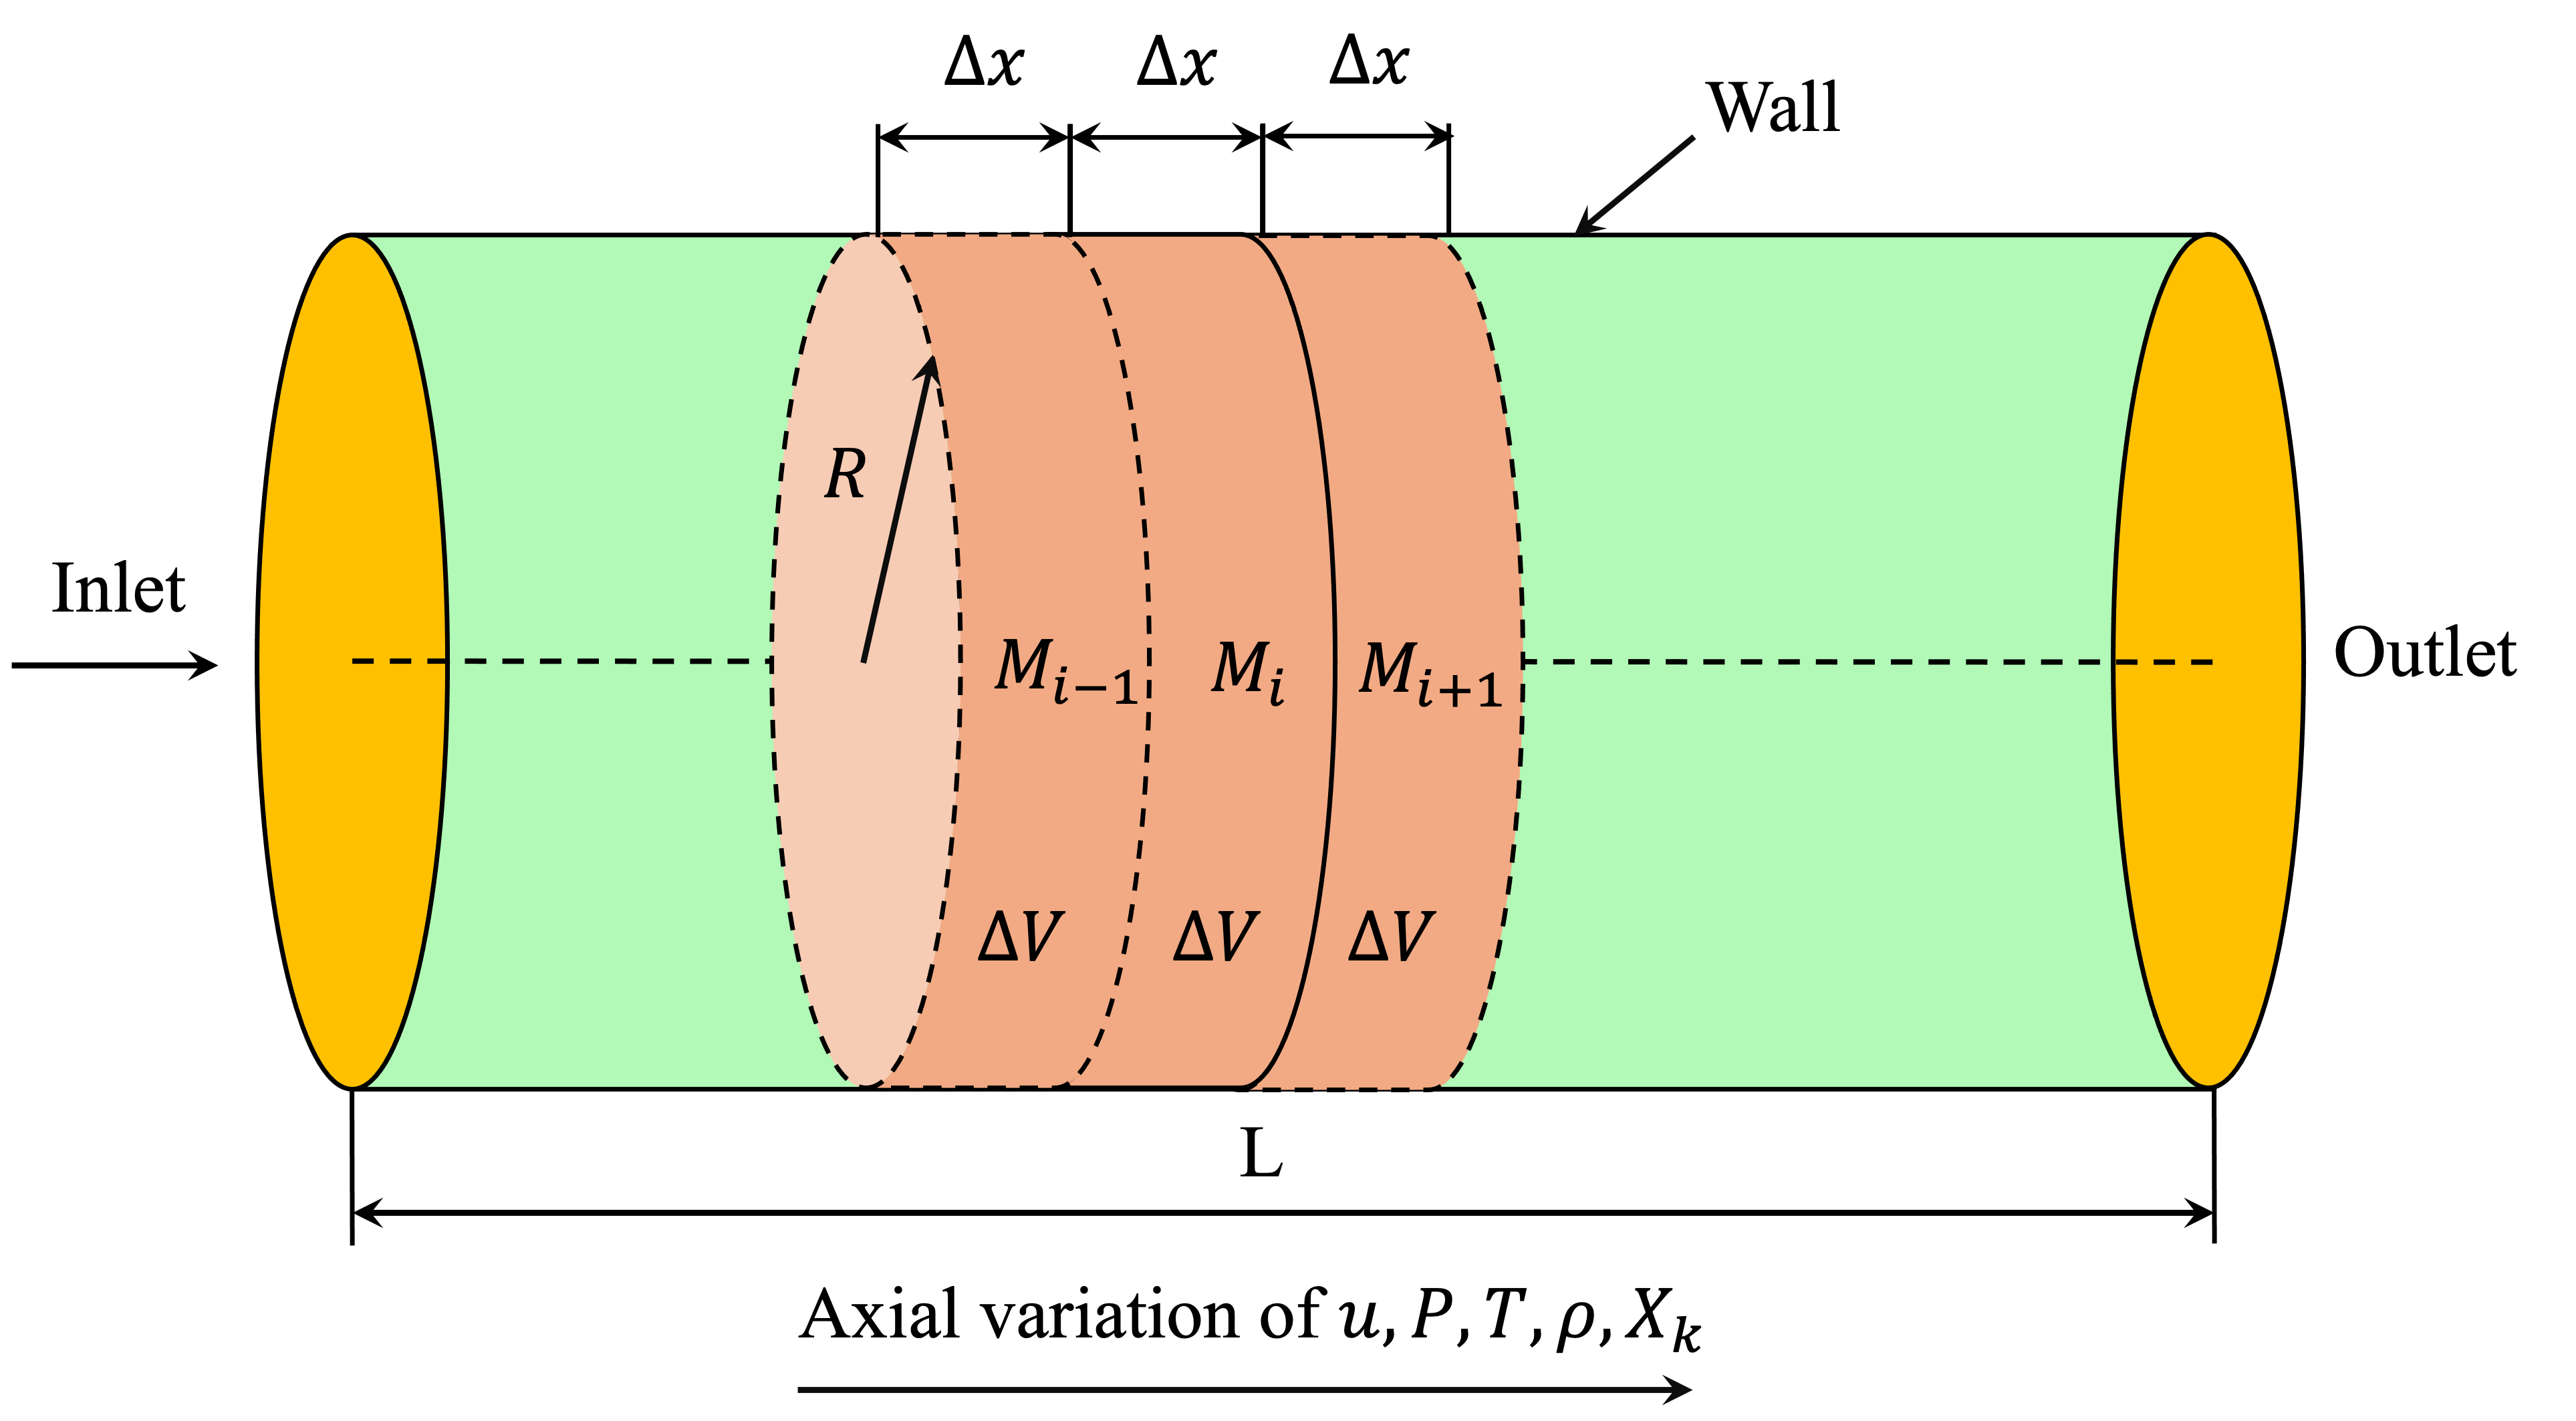
\includegraphics[width=0.61\textwidth]{PFR-schematic.png}
\caption{Schematic of a plug flow reactor-based representation of the hot-wall CVI reactor configuration. Here, $M_i$ denotes the $i^{th}$ plug along the axial ($x$) direction, and $\Delta x$, $\Delta V$, and $R$ denote the axial length, volume, and radius of the plug, respectively.}
\label{PFR-schematic}
\end{figure}

In this section, we first describe the details of the CVI reactor configuration. Afterward, the computational method is described. Finally, the details of the chemical mechanisms used in this study are presented.

\subsection{Details of the Setup}
\label{S:2.1}
We consider a cylindrical hot-wall flow CVI reactor configuration. A schematic of this reactor is shown in Fig. \ref{PFR-schematic}. The dimensions of the reactor follow a past study \cite{Dang2022}. The axial extent of the cylindrical reactor is $L = 0.52 \rm\ m$, and the inner radius is $R = 0.0048 \rm\ m$. At the inlet of the reactor, a premixed mixture of MTS, $\rm H_2$, and Ar enters at pressure $P$ and temperature $T$. The molar composition at the inlet of the reactor is 95\% Ar and 5\% mixture of MTS and $\rm H_2$. The ratio of molar composition of MTS and $\rm H_2$ is specified to be $\beta$, which is varied in this study from 0.05 to 0.2.

\subsection{Computational Approach}
\label{S:2.2}
The chemically reacting flow in the CVI reactor is simulated using a laminar PFR model. Such an approach has been followed in past studies for modeling the flow within CVD and CVI reactors \cite{Dang2022,Roman1995,Bammidipati1996}. A schematic of PFR is shown in Fig. \ref{PFR-schematic}. In a PFR, the steady laminar flow within a duct is modeled, where the gaseous flow in the transverse direction to the axial ($x$) direction is considered to be completely homogeneous. Therefore, changes in the state of the gas can only occur along the $x$ direction. Furthermore, in this modeling approach, all diffusion processes are neglected. As stated in \ref{S:1}, compared to a conventional CFD, even though a PFR is a much simpler representation of the flow, it can include detailed chemical kinetics, thus providing a computationally efficient approach for the simulation of physical phenomena such as pyrolysis, catalytic processes, and emissions.

A PFR is characterized by the state variables, which include density ($\rho$), temperature ($T$), pressure ($P$), mass fraction of $k^{\rm th}$ species, ($Y_k$) and the surface coverage of the $k^{\rm th}$ species ($S_k$). Here, we consider the net production of surface species to be zero, which implies the total surface coverage to be 1. The governing one-dimensional (1D) equations for PFR include conservation of mass, momentum, energy, and species mass equations, which are given by
\begin{align}
    u\frac{d\rho}{dx} + \rho\frac{du}{dx} & = 0, \tag{2.1} \\
    \rho u\frac{du}{dx} & = -\frac{dP}{dx}, \tag{2.2} \\
    \rho u c_{\rm p} \frac{dT}{dx} & = -\sum^N_{k=1} \overline h_k \dot \omega_k, \tag{2.3} \\
    \rho u \frac{dY_k}{dx} & = \dot \omega_k W_k, \qquad \textrm{for }\ k = 1,2,\dots,N. \tag{2.4}
\end{align}

\noindent Here, $c_{\rm p}$ denotes the specific heat of the mixture at constant pressure, $\overline h_k$ and $\dot\omega_k$ denote the molar enthalpy and reaction rate of the $k^{\rm th}$ species, respectively, and $N$ denotes the total number of species. These equations are further supplemented by the ideal gas equation of state
$\displaystyle \left ( \rho = \frac{P\overline W}{R_u T} \right )$
for relating the thermodynamic properties, and finite-rate chemical kinetics for determining $\dot\omega_k$. Here, $\overline W$ and $R_u$ denote the mixture molecular weight and universal gas constant, respectively. The system of governing equations is complete by specifying the inlet conditions. Note that, as the diffusion process is neglected, downstream parts of the reactor have no influence on upstream parts. Therefore, PFR can be integrated as initial value problems, starting from the composition at the inlet and moving towards the outlet by considering finite size volume ($\Delta V$), referred to as plugs, as shown in Fig. \ref{PFR-schematic}.

In the present study, the reactor length that is being considered here has a residence time of about 30 ms, which implies a negligible radial diffusion/stratification \cite{Dang2022}. Therefore, the PFR model utilizes a longer residence time of 500 ms than this critical limit. The PFR simulations are carried out using the Cantera
software \cite{Goodwin2014}, which is a well-established open-source software for the simulation of problems pertaining to thermodynamics, chemical kinetics, and transport processes.

\subsection{Chemical Kinetics Mechanisms}
\label{S:2.3}
We consider three chemical mechanisms with different levels of fidelity. These include a detailed 42 species and 103 steps mechanism \cite{Ge2007A,Ge2007B,Ge2010}, a moderately complex 20 species and 30 steps mechanism, and a globally reduced 5 species and 1 step mechanism \cite{Mousavipour2004}. Hereafter, these mechanisms are referred to as M1, M2, and M3, respectively. Here, the mechanism M1 serves as a reference for comparing the performance of the other two mechanisms. The globally reduced mechanism M3, as reported in past studies \cite{Dang2022,Mousavipour2004}, tends to be inadequate to describe the decomposition of MTS due to very few chemical species. The moderately complex mechanism M2 can be potentially useful for CFD and DSMC simulations, as it employs 20 species, which can potentially capture the effects of kinetics while still being cost-effective compared to the M1 mechanism. 

While M1 and M3 mechanisms are obtained from past studies, M2 is obtained by performing a reduction of the M1 mechanism using the Cantera software \cite{Goodwin2014}. The reduction strategy simulates an adiabatic constant pressure reactor over a range of pressure and temperature conditions relevant to this study, tracks the maximum reaction rates for each reaction, and identifies the important reactions based on the relative net reaction rate. This is followed by creating a series of reduced chemical mechanisms, including only the top reactions and the associated species, and performing the simulations again with these mechanisms to see whether the reduced mechanisms with a certain number of species are able to adequately simulate the reactor. The comparison of results from different reduced chemical mechanisms with the detailed M1 mechanism and dominant reactions obtained for major species using sensitivity analysis is discussed in Sec. \ref{S:3.1}.

\begin{table}[t] % FIXME: line breaks are not in same spot as original. why?
    \centering
    \caption{List of species in the M1, M2, and M3 chemical mechanisms.}
    \label{table:1}
    \begin{tabular}{ | p{0.11\textwidth}<{\centering} | p{0.8\textwidth}<{\centering}|}
        \hline
        Mechanism & Species \\
        \hline
        M1 & $\rm CH_3SiCl_3$, $\rm H_2$, $\rm CH_3$, $\rm SiCl_3$, $\rm H$, $\rm CH_2SiCl_3$, $\rm Cl$, $\rm CH_3SiCl_2$, $\rm CH_2SiCl_2$, $\rm HCl$, $\rm SiCl_2$, $\rm CH_2$, $\rm SiHCl_3$, $\rm CHSiCl_3$, $\rm CH_3SiCl$, $\rm Cl_2$, $\rm CH_4$, $\rm C_2H_5$, $\rm CH_2Cl$, $\rm CH_2Cl_2$, $\rm C_2H_4$, $\rm C_2H_2$, $\rm C_2H_3$, $\rm CH_2C$, $\rm CH_3C$, $\rm C_2H$, $\rm C_2H_5Cl$, $\rm C_2H_3Cl$, $\rm SiCl_4$, $\rm Si_2Cl_5$, $\rm Si_2Cl_4$, $\rm Si_2Cl_6$, $\rm SiHCl_2$, $\rm SiH_2Cl_2$, $\rm SiHCl$, $\rm SiH_2Cl$, $\rm SiH_3Cl$, $\rm CH_3SiHCl_2$, $\rm CH_2SiHCl$, $\rm C_2H_6$, $\rm CH_3SiH_2Cl$, $\rm Ar$ \\
        \hline
        M2 & $\rm SiCl_4$, $\rm CH_2SiCl_2$, $\rm H$, $\rm H_2$, $\rm SiHCl_3$, $\rm SiCl_2$, $\rm SiHCl_2$, $\rm SiCl_3$, $\rm HCl$, $\rm SiH_3Cl$, $\rm CH_2SiCl_3$, $\rm CH_4$, $\rm SiH_2Cl_2$, $\rm CH_3SiHCl_2$, $\rm CH_3SiCl_2$, $\rm CH_3$, $\rm Cl $, $\rm SiHCl$, $\rm CH_3SiCl_3$, $\rm Ar$ \\
        \hline
        M3 & $\rm CH_3SiCl_3$, $\rm H_2$, $\rm CH_4$, $\rm SiHCl_3$, $\rm Ar$ \\
        \hline
    \end{tabular}
\end{table}

\section{Assessment of Computational Strategy}
\label{S:3}
In this section, we first discuss the results from the reduction of the M1 mechanism yielding the M2 mechanism. Afterward, we compare the computational cost of the three mechanisms. Finally, we perform a verification and validation study using these mechanisms to establish the PFR-based strategy for further studies.

\subsection{Reduction of Chemical Mechanism}
\label{S:3.1}
To perform the reduction of the detailed mechanism M1, we simulate adiabatic constant-pressure reactors for 200 ms. We examine the accuracy of reduced mechanisms with increasing degree of complexity for a range of reactor temperatures (1100 K to 1600 K) and pressures (5 Torr to 100 Torr). The number of chemical reactions to be used in the reduced mechanism was varied from 10 to 50. As discussed in Sec. \ref{S:2.3}, the reduction strategy identifies the most active reactions. It resulted in mechanisms with the number of species varying from 12-28, with 10-50 reactions.

Figures \ref{T-vs-t-MTS} and \ref{T-vs-t-CH4} show the variation of mole fraction of MTS ($X_{\rm MTS}$) and CH$_4$ ($X_{\rm CH_4}$), respectively with respect to time. These species are chosen as they tend to be dominant species that participate in the homogeneous reactions and can further affect the heterogeneous surface reactions. At T = 1100 K, all reduced mechanisms with 10-20 reactions yield excellent agreement with the reference M1 mechanism at low (5 Torr) and high (100 Torr) pressure. The differences tend to occur only at higher temperatures (T = 1300 K and T = 1600 K), particularly with the reduced mechanism having 10 reactions. Such a difference with 10 reactions is observed for both MTS decomposition and CH$_4$ production. This can be attributed to enhanced decomposition/production of MTS/CH$_4$ at higher temperature, which is affected by the presence of reactions involving reactive intermediates when 20 or more reactions are included. At 1300 K, the pressure sensitivity is also observed as the error magnitude in the variation of $X_{\rm MTS}$ and $X_{\rm CH_4}$ with the 10-step mechanism is increased at higher pressure. At the highest temperature (T = 1600 K) and highest pressure ($P$ = 100 Torr), error is also observed with 20-step mechanisms. Based on these results, it can be inferred that a mechanism with 20 species and 30 reactions yields accurate results for the range of temperatures and pressures considered here. Therefore, for further studies, we consider the M2 mechanism to have 20 species and 30 reactions. Table \ref{table:1} lists all the species included in the three mechanisms. 

\begin{figure}[p] % FIXME: only using placeholder graphics
    \centering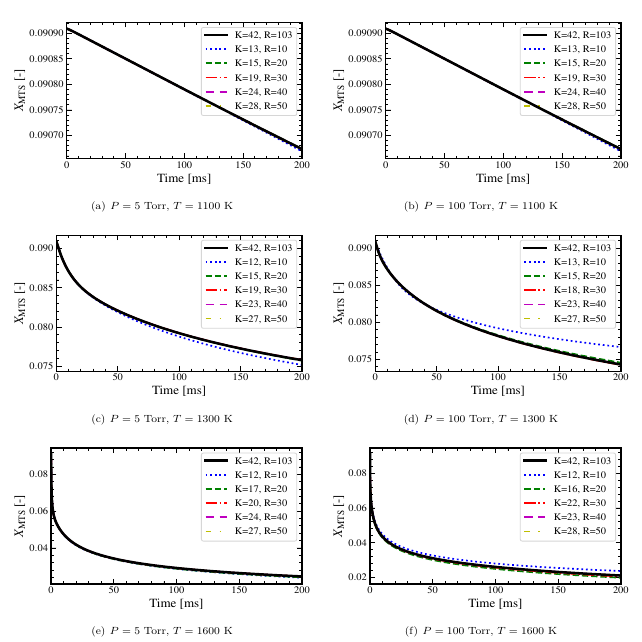
\includegraphics[width=\textwidth]{ph-fig2.png}
\caption{Comparison of time evolution of the mole fraction of MTS obtained using chemical mechanisms with different levels of complexity at T = 1100 K (a, b), T = 1300 K (c, d), and T = 1600 K (e, f) at P = 5 Torr (a, c, e) and P = 100 Torr (b, d, f). Here, K and R denotes the number of species and chemical reactions, respectively.}
\label{T-vs-t-MTS}
\end{figure}

\begin{figure}[p]
    \centering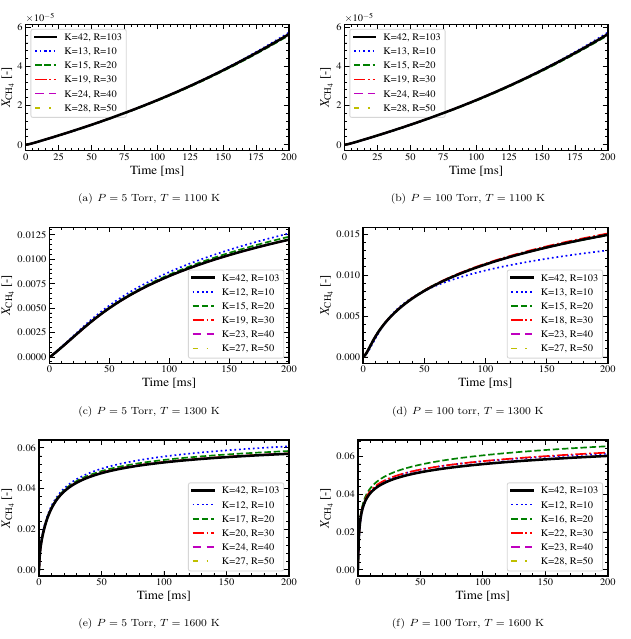
\includegraphics[width=\textwidth]{ph-fig3.png}
\caption{Comparison of time evolution of the mole fraction of CH$_4$ obtained using chemical mechanisms with different levels of complexity at T = 1100 K (a, b), T = 1300 K (c, d), and T = 1600 K (e, f) at P = 5 Torr (a, c, e) and P = 100 Torr (b, d, f). Here, K and R denotes the number of species and chemical reactions, respectively.}
\label{T-vs-t-CH4}
\end{figure}

\begin{figure}[tp] % FIXME: positioning of figures
    \centering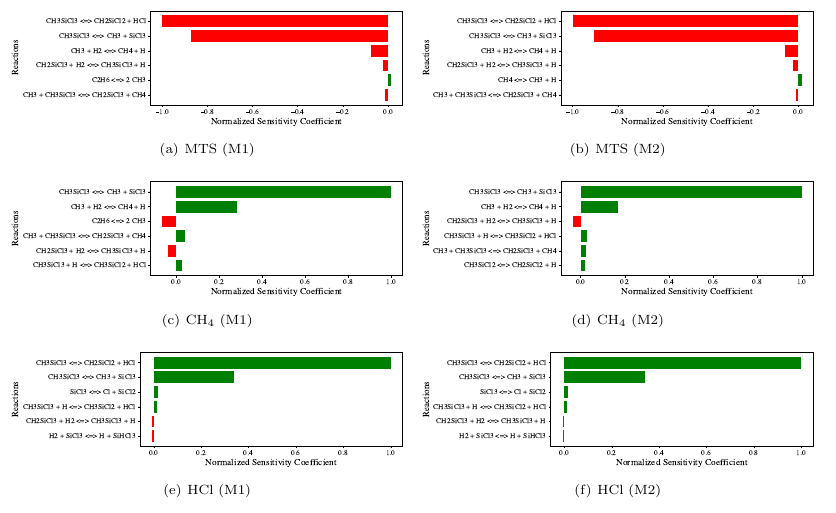
\includegraphics[width=\textwidth]{ph-fig4.png}
\caption{Six dominant reactions for MTS (a, b), CH$_4$ (c, d), and HCl (e, f) obtained using sensitivity analysis with M1 and M2 mechanisms.}
\label{Reactions-MTS-CH4-HCl}
\end{figure}

To further examine the dominant reactions corresponding to different species while using M1 and M2 mechanisms, a sensitivity analysis for different species is performed. The results from this analysis are shown in Fig. \ref{Reactions-MTS-CH4-HCl} for MTS, CH$_4$, and HCl. With both M1 and M2 mechanisms, the three dominant reactions are the same, which are given by
\begin{align} %FIXME: tags in original are not right aligned like these are
    \rm CH_3SiCl_3 \leftrightarrow CH_2SiCl_2 + HCl, & \tag{R1} \\
    \rm CH_3SiCl_3 \leftrightarrow CH_3 + SiCl_3, & \tag{R2} \\
    \rm CH_3 + H_2 \leftrightarrow CH_4 + H, & \tag{R3}
\end{align}

\noindent Out of these three reactions, MTS is more sensitive to R1 and R2. These reactions play a critical role in the decomposition of MTS and leads to formation of reactive intermediates such as $\rm CH_2SiCl_2$, CH$_3$, and SiCl$_3$, which can further decompose, combine, or participate in heterogeneous surface reactions. Additionally, R1 also leads to HCl, which is a byproduct responsible for gas-phase etching \cite{Wang2008,Guan2020}. The R3 reaction is primarily responsible for the formation of CH$_4$, which can help avoid contamination, and the radical H, which is crucial for the removal of Cl and the promotion of SiC growth through heterogeneous reactions \cite{Brennan1990}. 

For CH$_4$, R1 and R3 are the first two dominant reactions (see Fig. \ref{Reactions-MTS-CH4-HCl}(c) and (d)), which are found in both M1 and M2 mechanisms. However, the third dominant reaction is different for CH$_4$ with M1 and M2 mechanisms. While the M1 mechanism shows the third dominant reaction to be decomposition of $\rm C_2H_6$ into CH$_3$ radical through the reaction
\begin{align*}
    \rm C_2H_6 \leftrightarrow 2CH_3,
\end{align*}
the M2 mechanism shows the third dominant reaction as:
\begin{align*}
    \rm CH_2SiCL_3 + H2 \leftrightarrow CH_3SiCl_3 + H.
\end{align*}
This difference could be due to the absence of $\rm C_2H_6$ in the M2 mechanism (see Table \ref{table:1}). Although the third dominant reaction for CH$_4$ differs for the M1 and M2 mechanisms, the sensitivity of the first two dominant reactions is much higher compared to the third reaction.

An important byproduct during the decomposition of MTS is HCl. With both M1 and M2 mechanisms, similar to MTS, R1 and R2 are the first two dominant reactions (see Fig. \ref{Reactions-MTS-CH4-HCl}(e) and (f)), whereas the third dominant reaction is
\begin{align*}
    \rm SiCl_3 \leftrightarrow SiCl_2 + Cl.
\end{align*}
This is an intermediate and critical reaction, as SiCl$_2$ is a direct precursor to SiC formation via heterogeneous reaction with H$_2$ or CH$_2$ at the surface \cite{Papasouliotis1994}. On the other hand, the radical Cl can either react with H$_2$, leading to the formation of HCl, which in turn can prevent the formation of the undesirable Cl-rich byproducts such as SiCl$_4$.

To summarize, the results discussed in this section from the adiabatic reactor simulations and sensitivity analysis demonstrate that the reduced M2 mechanism can be considered adequate to capture the key aspects of MTS decomposition in the presence of H$_2$ in comparison to the detailed M1 mechanism for the conditions relevant to this study.

\subsection{Computational Cost}
As the number of species and reactions tends to differ in the three chemical mechanisms, it is expected that the computational cost will differ. A key focus of the present work is to demonstrate that moderately complex chemical kinetics, such as the M2 mechanism, can yield accurate results, which in turn can be used with CFD simulations. Here, we assess the computational cost of the three mechanisms by simulating a PFR at a pressure of 5 Torr and a temperature of 1350 K. The computational cost comparison is shown in Table \ref{table:2}.

\begin{table}[t]
    \centering
    \caption{Comparison of computational cost for 1 PFR simulation using M1, M2, and M3 mechanisms.}
    \label{table:2}
    \begin{tabular}{ | c | c | c | }
        \hline
        Mechanism & Computational Cost [s] & Relative Cost [\%] \\
        \hline
        M1 & 10.4 & 100 \\
        M2 & 4.6 & 44.2 \\
        M3 & 2.7 & 26 \\
        \hline
    \end{tabular}
\end{table}

As expected, the computational cost of the M2 and M3 mechanisms is lower than the detailed M1 mechanism. The cost of M2 decreases primarily due to a decrease in the number of species compared to M1, from 42 to 20, with a much less impact of a decrease in the number of reactions. Note that mechanisms such as M2 can be used for CFD simulations, as mechanisms with 15-20 chemical species tend to be manageable while employing finite-rate kinetics. However, it should be noted that the cost of a CFD simulation, apart from including the kinetics cost, also includes the cost of computation of convective and diffusive fluxes, which can be comparable to or larger than the cost of kinetics compared to a PFR simulation. The cost of M3 does not linearly scale with the number of species, which can be associated with a reduced rate of convergence of the PFR simulation with the M1 mechanism.

\subsection{Verification and Validation}
\begin{figure}[t] % FIXME: only using placeholder graphics
    \centering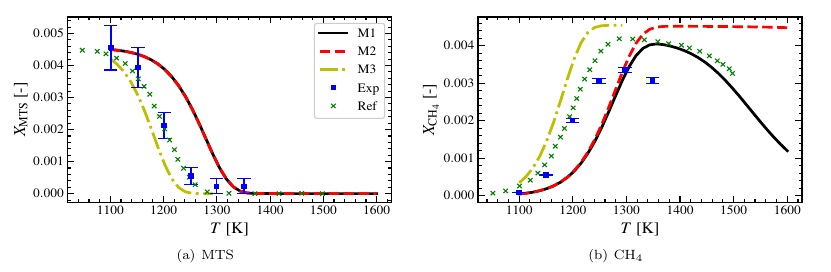
\includegraphics[width=\textwidth]{ph-fig5.png}
    \caption{Variation of mole fraction of MTS (a) and CH$_4$ (b) with respect to temperature. Experimental data and ‘Ref‘ data corresponds to experimental and computational study using detailed mechanism \cite{Dang2022}.}
    \label{fig:5}
\end{figure}

We perform the verification and validation of the PFR-based strategy by simulating MTS decomposition in the presence of H$_2$ at an operating pressure of 1 atm (760 Torr), inlet composition ratio of 0.1, and over a range of temperatures varying from 1100 K to 1600 K. The results are compared in Fig. \ref{fig:5}, which includes the variation of the mole fraction of MTS and CH$_4$ with respect to temperature. For comparison, we also include experimental and computational results obtained using a detailed chemical mechanism from a past study \cite{Dang2022}. Note that the detailed mechanism used in the reference study was devised to match the experimental data. Furthermore, the operating pressure of the present configuration is much higher than that of a typical CVI, which is usually operated at lower pressures. 

Both M1 and M2 mechanisms yield the same results for MTS, which starts to decompose gradually from 1100 K to 1200 K, and then rapidly leads to a nearly complete decomposition by 1350 K. The values of MTS by these mechanisms are over-predicted compared to the reference results. Although the rate of decomposition of MTS from the M1 and M3 mechanisms matches during early and later stages with the reference computational results, the decomposition of MTS is delayed with respect to temperature. The results from the M3 mechanism are under-predicted compared to the reference results and show an early and faster rate of decomposition of MTS. Typically, one-step mechanisms, such as the M3 mechanism, are devised so that the variation of major species is captured well, which is not the case here, thus indicating its inaccuracy.

The results for the variation of CH4 mole fraction (see Fig. \ref{fig:5}(b)) from the M1 and M2 mechanisms tend to match till 1350 K. At temperatures beyond 1350 K, the M1 mechanism show reduced levels of CH$_4$ implying its further decomposition, whereas the M2 mechanism yields constant values of CH$_4$. The differences can be attributed to the effects of reduced number of species and reactions in the M2 mechanism compared to the M1 mechanism, which can affect the thermodynamics and reaction pathways. However, for typical CVI conditions of 800 to 1000 $^o$C, both mechanisms yield similar results, implying M2 can be considered to be accurate with respect to M1. As Fig. \ref{fig:5}(a) showed a delayed decomposition of MTS with respect to temperature using M1 and M2 mechanisms, this leads to a delayed production of CH$_4$ compared to the reference results. The peak value of CH$_4$ and its variation at higher temperatures by the M1 mechanism show good agreement with the reference computational results. Compared to experimental data, the peak values of CH$_4$ are over-predicted by all mechanisms. With the M3 mechanism, the production of CH$_4$ is over-predicted as it correlates with the under-prediction of MTS in Fig. \ref{fig:5}(a).

The results shown here demonstrate that the PFR strategy employed here can capture the decomposition of MTS in the presence of H$_2$. There are differences in the results from the detailed M1 mechanism and the detailed mechanism proposed in the reference study \cite{Dang2022}, which was devised to capture the experimental results. However, these differences are associated with a delayed start of decomposition of MTS and pro- duction of CH$_4$ with respect to temperature, although the rates of decomposition of MTS and production of CH$_4$ tend to match. In this study, we have not made any attempts to modify the baseline M1 mechanism, as the experimental data is only available at 760 Torr, whereas this study examines CVI reactor configurations at lower pressures. Therefore, the results from the M1 mechanism are considered as a reference in the rest of this study to examine the effects of operating conditions on the MTS decomposition and to assess the performance of the M2 and M3 mechanisms.

\section{Results and Discussion}
In this section, we discuss the results obtained from the PFR simulations of the MTS/H$_2$ decomposition under a wide range of CVI-relevant operating conditions. First, we analyze the effects of operating temperature at different values of pressure. Afterward, we examine the effects of operating pressure at different values of temperature. This is followed by the analysis of results from the cases employing temperature and pressure gradients at different values of pressures and temperatures. Finally, the effects of the molar ratio of MTS to H$_2$ ($\beta$) at the inlet of the CVI reactor are examined under two reactor configurations, which include isothermal and temperature-gradient conditions across the reactor for optimal operating pressure and temperature conditions.

In a CVI relevant conditions, the decomposition of MTS/H$_2$ leads to the formation of several intermediate reactive species. We examine the concentration of several species, such as MTS, CH$_4$, SiHCl$_3$, SiCl$_4$, HCl, and SiCl$_2$, some of which also participate in the heterogeneous surface reactions. At high temperatures, CH$_4$ produced during the decomposition of MTS can further decompose through thermal cracking providing a source of carbon \cite{Golecki2003}, which depending upon the operating conditions can contribute to SiC formation \cite{Aarnaes2020}, or can lead to unwanted residual carbon \cite{Ksiazek2014,Aarnaes2022}. Furthermore, it acts as a diluent to the reactive gas phase, as it can also compete with MTS. The hydrogenation of the Si-C bond in MTS and substitution of methyl (CH$_3$) radical with H$_2$ leads to the formation of SiHCl$_3$. It is a reactive intermediate that can further decompose, providing the Si needed for the SiC deposition. It can also react further, leading to HCl, and can affect the deposition rate. However, if SiHCl$_3$ does not react further, it can carry silicon away from the deposition zone, which can lower the SiC yield or lead to a Si-deficient or C-rich matrix. SiCl$_4$ is also a dominant and stable species, which is generally inactive toward SiC formation under typical CVI conditions, however, it can act as a source of the Si \cite{Dang2022,Hu2019}. It can also affect the gas-phase equilibrium, overall Si/C balance, and deposition kinetics. SiCl$_2$ is a highly reactive intermediate, which serves as a key Si-bearing species that readily reacts with carbon-containing gases such as CH$_4$, $\rm C_2H_2$, or CH$_2$ to form solid SiC. For example, the following heterogeneous reaction leads to the formation of SiC \cite{Papasouliotis1994}:
\begin{align*}
    \rm SiCl_2(g) + CH_2(g) \rightarrow SiC(s) + 2HCl(g)
\end{align*}
Due to its high reactivity, SiCl$_2$ promotes rapid SiC growth near the infiltration front, enhancing deposition efficiency. However, excessive SiCl$_2$ may lead to non-uniform deposition or pore closure. Finally, HCl is produced as a major gaseous species, which, although it does not participate directly in SiC formation, can potentially shift the chemical equilibria, suppressing undesirable gas-phase nucleation and enhancing deposition selectivity on solid surfaces.

It is evident that the aforementioned species play a crucial role in affecting the Si:C ratio, shifting of the gas-phase equilibrium, and the deposition kinetics, which in turn affect the SiC deposition while including the heterogeneous surface reactions. Therefore, we examine the concentration of all these species in the subsequent discussion of results. Here onwards, the molar composition of the species is obtained at the exit of the reactor and each PFR simulation, as discussed before in Sec. \ref{S:2.2}, is carried out for a residence time of 500 ms within the reactor.

\subsection{Effects of Temperature}
\label{S:4.1}
To examine the effects of operating temperature ($T$), we simulate the PFR over a range of values of $T$ from 1100 K to 1600 K. Additionally, each PFR simulation is performed at three values of operating pressure ($P$), which include 5 Torr, 52.5 Torr, and 100 Torr. From these simulations, the mole fraction of several of the species is obtained at the exit of the reactor, which are shown in Fig. \ref{fig:6}.

It is evident from Fig. \ref{fig:6}(a) that MTS tends to decompose at a slower rate for $T$ varying from 1100 to about 1180 K with both M1 and M2 mechanisms. However, beyond this value of $T$, it tends to decompose at a higher rate. For $T$ > 1350 K, no MTS is observed at the exit of the PFR, implying its complete decomposition. These results are consistent with the past studies conducted at different pressure values \cite{Dang2022,Peng2021,Yang2009}, which have also shown that MTS in the presence of H$_2$ starts to decompose around $T\approx$ 1100 K and the rate of decomposition increases with an increase in $T$. Both M1 and M2 mechanisms yield identical results, however, the globally reduced M3 mechanism leads to a significant over-prediction of MTS.
\begin{figure}[p]
    \centering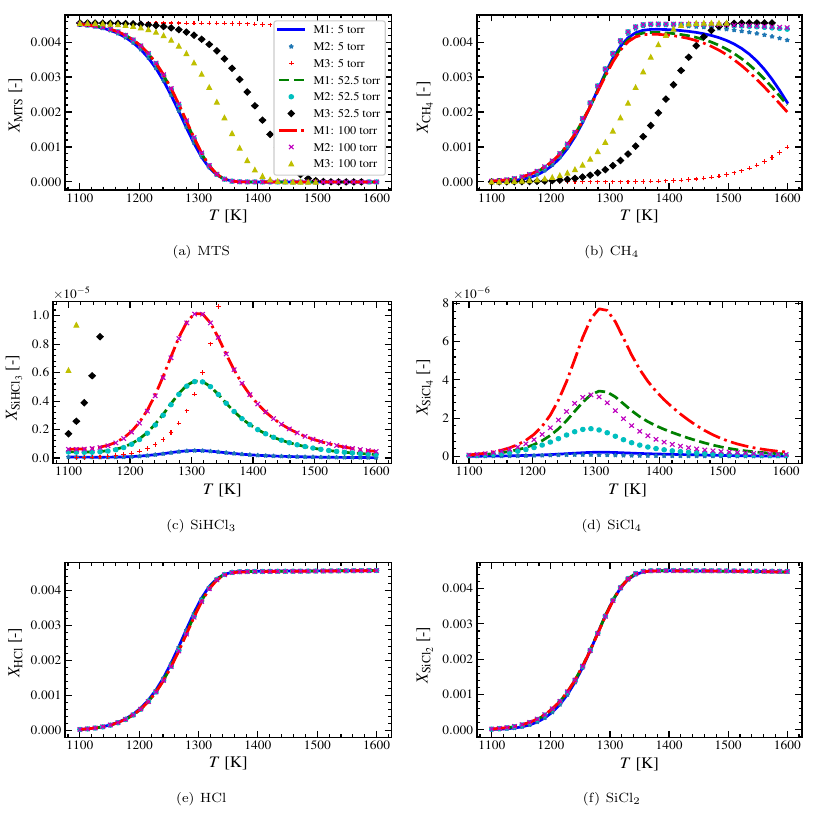
\includegraphics[width=\textwidth]{ph-fig6.png}
    \caption{Variation of mole fraction of MTS (a), CH$_4$ (b), SiHCl$_3$ (c), SiCl$_4$ (d), HCl (e), and SiCl$_2$ (f) with respect to temperature at three values of operating pressure (5 Torr, 52.5 Torr, and 100 Torr).}
    \label{fig:6}
\end{figure}
Furthermore, with M1 and M2 mechanisms, we do not observe any sensitivity of the results to $P$. However, the sensitivity to $P$ is evident in the results using the M3 mechanism, where in the case with $P$ = 5 Torr, the decomposition of MTS tends to be incomplete even at $T$ = 1600 K.

The variation of $X_{\rm CH_4}$ with respect to $T$ in Fig. \ref{fig:6}(b) shows that it tends to increase with $T$, reaching a peak value at around 1350 K. The peak value shows a minor decrease with an increase in $P$. This behavior is captured by both mechanisms M1 and M2. However, a further increase in the value of $T$ shows differences in the results from the M1 and M2 mechanisms. While a decrease in $X_{\rm CH_4}$ with respect to $T$ occurs with the M1 mechanism, the M2 mechanism yields nearly constant values. The rate of decrease of $X_{\rm CH_4}$ with mechanism M1 increases with an increase in $P$. As discussed before, CH$_4$ can play a critical role in the SiC deposition process, as its further decomposition can provide a source of carbon, which, depending upon conditions, can contribute to SiC formation or can lead to unwanted residual carbon. At around $T$ = 1200 to 1300 K,
$X_{\rm MTS}/X_{\rm CH_4} \lessapprox 1$, which is considered suitable for promoting stoichiometric SiC formation. From these results, we can also infer that M2 can be considered to yield reasonable agreement with M1 till $T \approx$ 1400 K. The results from the globally reduced M3 mechanism differ substantially from the other two mechanisms. As MTS tends to decompose at higher values of $T$ (see Fig. \ref{fig:6}(a)), it affects the production of CH$_4$. Furthermore, similar to the sensitivity of MTS decomposition, the sensitivity of CH$_4$ production/consumption to $P$ is also evident, particularly at the lower pressure.

The variation of $X_{\rm SiHCl_3}$ and $X_{\rm SiCl_4}$ shown in Figs. \ref{fig:6}(c) and (d) with respect to $T$ tends to be similar with mechanisms M1 and M2. It is observed that their values increase with $T$ and attain a maximum around $T$ = 1300 K, which is followed by a decrease with a further increase in $T$. The sensitivity to $P$ is clearly evident, where we observe that the peak value increases with $P$. The differences between M1 and M2 tend to occur in the variation of $X_{\rm SiCl_4}$, where the peak values by M2 are under-predicted. However, compared to other chemical species, the quantitative value of $X_{\rm SiCl_4}$ tends to be an order of magnitude smaller. With the M3 mechanism, the peak value of $X_{\rm SiHCl_3}$ is significantly over-predicted compared to the other two mechanisms. As discussed before, SiHCl$_3$ is a parasitic byproduct, which carries Si away from the deposition zone, which can lower the SiC yield or lead to a Si-deficient or C-rich matrix. Therefore, using the M3 mechanism can lead to inaccurate prediction of SiC deposition.

Both HCl and SiCl$_2$ show a similar variation with $T$ (see Figs. \ref{fig:6}(e) and (f)), where we can observe an increase with $T$ till about 1350 K, which is followed by nearly constant values with $T$. Furthermore, there is no sensitivity to $P$ and both mechanisms yield the same results, again demonstrating the accuracy of the M2 mechanism. As discussed before, both HCl and SiCl$_2$ can be advantageous for SiC deposition, however, their excess composition should be avoided. From the results, we can infer that $T <$ 1300 K leads to $X_{\rm HCl}$ and $X_{\rm SiCl_2}$ less than their corresponding maximum values.

Based on the results discussed in this section for the effects of $T$, we can infer that 1250 K $\lessapprox T \lessapprox$ 1300 K can be considered a reasonable range for the operating temperature of the reactor. In this range of $T$, the decomposition of MTS is adequate, and the formation of byproducts is lower than their corresponding peak values. Furthermore, the M2 mechanism tends to yield comparable results to those obtained using the M1 mechanism, while the M3 mechanism, as expected, tends to yield inaccurate results. The sensitivity to $P$ is evident on several of the byproducts during the decomposition of MTS, which is discussed further in the next section.

\subsection{Effects of Pressure}
\label{S:4.2}
\begin{figure}[p]
    \centering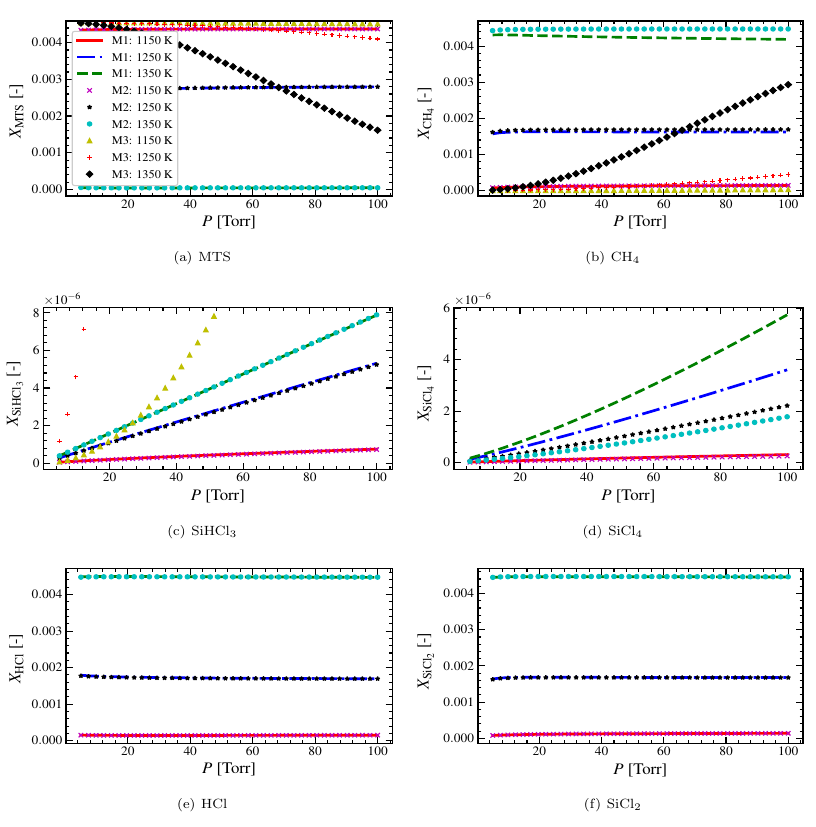
\includegraphics[width=\textwidth]{ph-fig7.png}
    \caption{Variation of mole fraction of MTS (a), CH$_4$ (b), SiHCl$_3$ (c), SiCl$_4$ (d), HCl (e), and SiCl$_2$ (f) with respect to pressure at three values of operating temperature (1150 K, 1250 K, and 1350 K).}
    \label{fig:7}
\end{figure}

We examine the effects of $P$ by varying it from 5 to 100 Torr at three different values of $T$. Based on the results discussed in Sec. \ref{S:4.1}, we observe that the major species showed significant variation for $T$ within the range of 1150-1350 K, therefore, we consider three values of $T$, namely, 1150 K, 1250 K, and 1350 K. Figure \ref{fig:7} shows the variation of mole fraction of six species with respect to $P$ at the exit of the reactor. 

We can observe in Figs. \ref{fig:7}(a) and (b) that both MTS and CH$_4$ do not show much sensitivity to the variation in $P$, particularly while using M1 and M2 mechanisms. Past studies under CVD conditions have also shown weak sensitivity to $P$ on the decomposition under typical pyrolysis conditions (800-1400 $^o$C). However, the M3 mechanism does exhibit the effects of pressure, which leads to an increase in decomposition/production of MTS/CH$_4$ , particularly at higher temperatures (1250 K and 1350 K). This again shows the inaccuracy of the globally reduced mechanism. 

The variation of other species such as SiHCl$_3$ and SiCl$_4$ (see Figs. \ref{fig:7}(c) and (d)) does exhibit sensitivity to the variation of $P$ with all three mechanisms. The mole fraction of these species tends to increase with $P$ at all three values of $T$, although the increase in $T$ leads to an augmentation of the rate of increase of production of these species with $P$. Such an increase in the production of SiHCl$_3$ with an increase in $P$ is due to its formation pathway being governed by gas-phase equilibrium reactions and radical-driven mechanisms. For example, SiHCl$_3$ is generated via the secondary gas-phase reactions involving MTS fragments and HCl through the following reactions
\begin{align*}
    \rm CHSiCl_3 \rightarrow CH_3 + SiCl_3 \quad (\textrm{Pyrolysis step}), & \\
    \rm SiCl_3 + HCl \leftrightarrow SiHCl_3 + Cl \quad (\textrm{Equilibrium limited step}). &
\end{align*}
In the above equations, the equilibrium is sensitive to $P$, as a higher value of $P$ shifts the equilibrium toward fewer gas-phase species and a lower value of $P$ suppresses reverse reactions, reducing SiHCl$_3$ yield. Moreover, the gas-phase radicals, such as SiCl$_3$ and CH$_3$ persist longer due to fewer collisions at lower pressure ($P$ < 10 Torr), whereas at higher $P$, the increased collision frequency promotes radical recombination, enhancing the production of SiHCl$_3$ . For similar reasons, the production of SiCl$_4$ increases with $P$ as its formation is also governed by gas-phase equilibrium reactions and chlorine redistribution pathways. While the M2 mechanism shows excellent agreement with the M1 mechanism for the production of SiHCl$_3$ , it tends to underpredict the production of SiCl$_4$ , particularly at $T$ = 1250 K and 1350 K. This discrepancy can be attributed to the absence of the following reaction from the M2 mechanism, which is another pathway of production of SiCl$_4$
\begin{align*}
    \rm SiCl_3 + HCl \leftrightarrow SiCl_4 + H \quad (\textrm{Equilibrium limited step}). &
\end{align*}
The M3 mechanism shows significant overprediction of SiHCl$_3$ , which again underscores its inaccuracy.

Unlike SiHCl$_3$ and SiCl$_4$, and similar to MTS and CH$_4$ , the mole fractions of HCl and SiCl$_2$ exhibit insensitivity to $P$ at the three values of $T$. The production of HCl primarily depends upon temperature and mass flow rate/residence time. Similarly, the production of SiCl2 shows insensitivity to $P$ as it is a short-lived intermediate species, and its formation is governed by unimolecular decomposition of MTS or its fragments. For example, one reaction pathway for the production of SiCl$_2$ is
\begin{align*}
    \rm SiCl_3 \leftrightarrow SiCl_2 + Cl, &
\end{align*}
which quickly reacts with H$_2$ or Cl, leaving its steady-state concentration kinetically controlled, not equilibrium-limited, and thus the observed pressure insensitivity. Past experimental studies have also shown that SiCl$_2$ concentrations remain constant across 1–100 Torr for a fixed ratio of MTS/H$_2$. It has been observed that only for $P$ < 0.1 Torr, the production of SiCl$_2$ decreases with $P$ due to reduced collision frequency.

Overall, the results in this section illustrate that the sensitivity of the mole fraction of various chemical species under CVI-relevant conditions is highly dependent upon the reaction pathways. If the production of a particular species is dependent upon equilibrium-limited reaction or radical recombination, the sensitivity to the pressure is observed. Otherwise, the unimolecular production of species is directly dependent upon MTS decomposition, which, under the range of conditions considered here, shows no sensitivity to the pressure
variation.

\subsection{Effects of Temperature Gradient}
\begin{figure}[p]
    \centering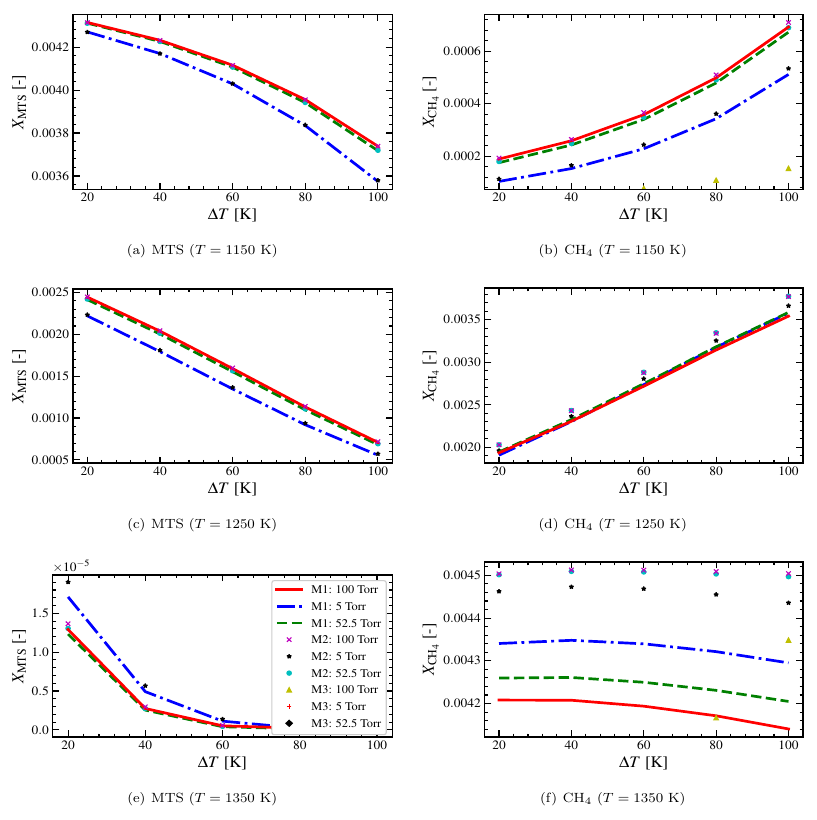
\includegraphics[width=\textwidth]{ph-fig8.png}
    \caption{Variation of mole fraction of MTS (a, c, e) and CH$_4$ (b, d, f) with respect to the temperature gradient at three values of operating pressure (5 Torr, 52.5 Torr, and 100 Torr) at inlet temperature of 1150 K (a, b), 1250 K (c, d), and 1350 K (e, f). The results from the M3 mechanism are not visible in these figures as they are significantly over-predicted for MTS and under-predicted for CH$_4$.}
    \label{fig:8}
\end{figure}
\begin{figure}[p]
    \centering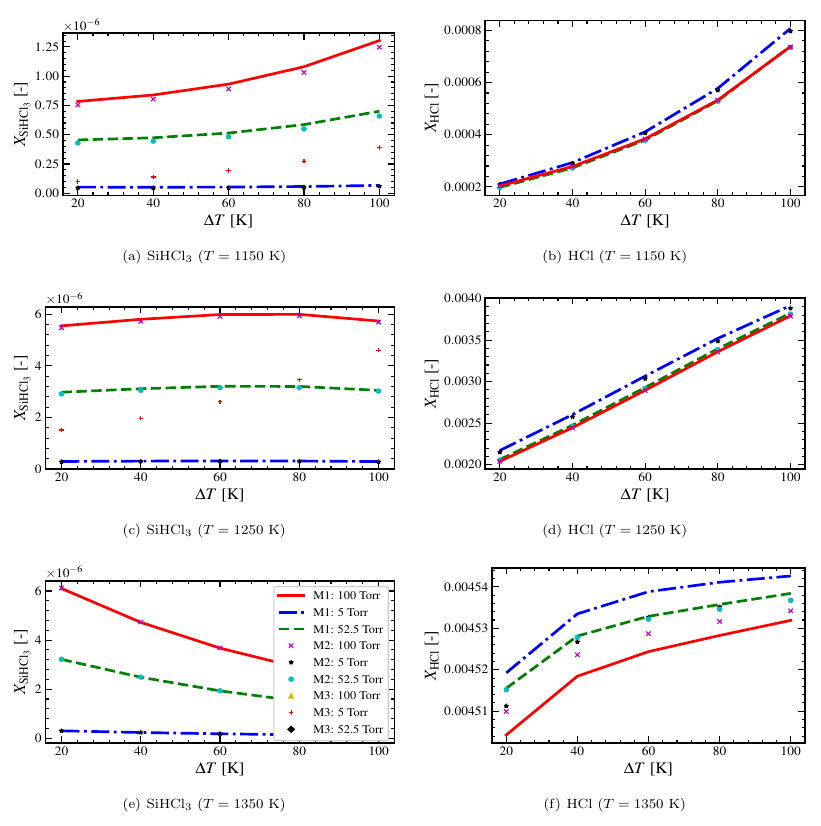
\includegraphics[width=\textwidth]{ph-fig9.png}
    \caption{Variation of mole fraction of SiHCl$_3$ (a, c, e) and HCl (b, d, f) with respect to the temperature gradient at three values of operating pressure (5 Torr, 52.5 Torr, and 100 Torr) at inlet temperature of 1150 K (a, b), 1250 K (c, d), and 1350 K (e, f). Some of the results from the M3 mechanism are not visible in these figures as they are significantly over- or under-predicted compared to the M1 and M2 mechanisms.}
    \label{fig:9}
\end{figure}
Now, we examine the effects of temperature gradient ($dT/dx$) on the decomposition process. We consider temperature variation (drop) of 10 K to 100 K across the reactor length, $L$, at different inlet temperatures (1150 K, 1250 K, 1350 K) at three values of operating pressure (5 Torr, 52.5 Torr, and 100 Torr). These conditions imply that the temperature gradient, $dT/dx$, varies from about -190 K/m to -19 K/m.

At $T$ = 1150K, the decomposition of MTS starts leading to a decrease in its value and the production of byproducts such as CH$_4$ (see Fig. \ref{fig:6}(a) and (b)). However, the decomposition/production of MTS/CH$_4$ is en hanced due to the presence of a temperature gradient. The rate of increase of the decomposition/production of MTS/CH$_4$ tends to a constant value with an increase in $P$. Both M1 and M2 mechanisms yield the same results, while the M3 mechanism fails to predict the decomposition/production of MTS/CH$_4$ at this temperature.

The enhanced decomposition of MTS is due to the combined thermodynamics and kinetics effects. A hot inlet and cold outlet lead to a thermodynamic driving of the endothermic decomposition of MTS. Additionally, the Arrhenius kinetics get accelerated near the hot inlet, thus enhancing the decomposition. The byproducts, such as CH$_4$ and HCl, are driven towards the cooler outlet zone, which also facilitates the decomposition of MTS in the hot zone. The production of CH$_4$ is also enhanced with an increase in $|dT/dx|$ due to combined thermodynamics and kinetics effects. For example, after decomposition of MTS in high temperature zones into radicals such as CH$_3$ and the decomposition of H$_2$ into H, CH$_4$ tends to form through the radical recombination reaction, such as
%eqn
Note that CH$_4$ is thermodynamically stable at lower temperatures. Lastly, some of the competing reaction pathways are suppressed due to the presence of a temperature gradient. For example, without the presence of a temperature gradient, CH$_3$ can polymerize to form C$_2$H$_6$, whereas with a temperature gradient, CH$_4$ can be removed rapidly to the low temperature region, leading to its enhanced production.

At $T$ = 1250 K and 1350 K, the decomposition/production of MTS/CH$_4$ is enhanced further, which is expected as evident from Fig. \ref{fig:8}. However, the dependence of MTS and CH$_4$ mole fractions on $\Delta T$ changes significantly as the inlet temperature is changed. At 1150 K, the decomposition of MTS increases with $\Delta T$ gradually, while at 1250 K, a linear dependence on $\Delta T$ is observed, and at 1350 K, a rapid decomposition of MTS occurs even with low temperature gradients. This is primarily due to kinetic effects. The dependence of CH$_4$, although showing similar trends at 1150 and 1250 K, at 1350 K, its value tends to decrease with $\Delta T$ in a weak manner.

The results from the M2 mechanism at $T$ = 1250 K and 1350 K compare well with the M1 mechanism for the production of MTS. However, we can observe overprediction in the production of CH$_4$, particularly at $T$ = 1350 K, which also shows sensitivity to $P$. As discussed before in Sec. \ref{S:4.1}, the production of CH$_4$ by the M2 mechanism showed overprediction compared to the M1 mechanism, which can be attributed to the absence of some of the reaction pathways, where CH$_4$ is involved, and the absence of some of the chemical species in this mechanism. Even at 1350 K, the results from M3 are significantly inaccurate for both MTS and CH$_4$ compared to the M1 mechanism.

Figure \ref{fig:9} shows the effects of variation in $\Delta T$ on two other byproducts, namely, SiHCl$_3$ and HCl. As the qualitative variation of SiCl$_4$ and SiCl$_2$ with respect to the $\Delta T$ was observed to be similar to SiHCl$_3$ and HCl, respectively, the variation of mole fraction of these species is not shown here for the sake of brevity. The dependence of SiHCl$_3$ production exhibits a complex behavior with respect to $\Delta T$ at different values of the inlet temperature, which can be attributed to the presence of multiple pathways of its formation and the effects of kinetics and thermodynamics. While at 1150 K, the production of SiHCl$_3$ is enhanced, at 1350 K, it reduces with respect to $\Delta T$ . On the other hand, at 1250 K, SiHCl$_3$ production is marginally enhanced till $\Delta T \approx$ 80 K, and afterwards a decrease in the production is observed. The effect of pressure is also evident, which leads to higher levels of production of SiHCl$_3$ at high pressure due to the dominance of recombination reactions.

The production of HCl is enhanced with an increase in $\Delta T$ at all inlet temperatures, although the dependence on $\Delta T$ shows different behavior at different inlet temperatures. While at 1150 K, the rate of increase of the production of HCl with $\Delta T$ increases, at 1250 K, it stays nearly constant, and at 1350 K, it tends to decrease. Furthermore, the effect of pressure is also evident, which shows a decrease in the production of HCl at higher pressure. The observed variation of production of HCl with an increase in $\Delta T$ underscores the role played by thermodynamics, kinetics, and transport. For example, higher temperature leads to enhanced decomposition of MTS, which facilitates the production of HCl. At lower temperatures, HCl tends to be thermodynamically stable, and thus, the reactions that consume HCl get limited. The temperature gradient also ensures that the produced HCl in the hot zones is convected to the low temperature exhaust zone. Lastly, even though HCl production is insensitive to pressure, low pressure enhances HCl evacuation to low temperature zones.

To summarize, the presence of a temperature gradient favors the decomposition of MTS, which in turn leads to the production of the byproducts. However, the effect of operating temperature leads to a complex dependence of the mole fraction of the species on the temperature gradient, which highlights the effects of kinetics, thermodynamics, and transport processes, and the presence of multiple pathways for the formation of several intermediate reactive species.

\subsection{Effects of Pressure Gradient}
\begin{figure}[p]
    \centering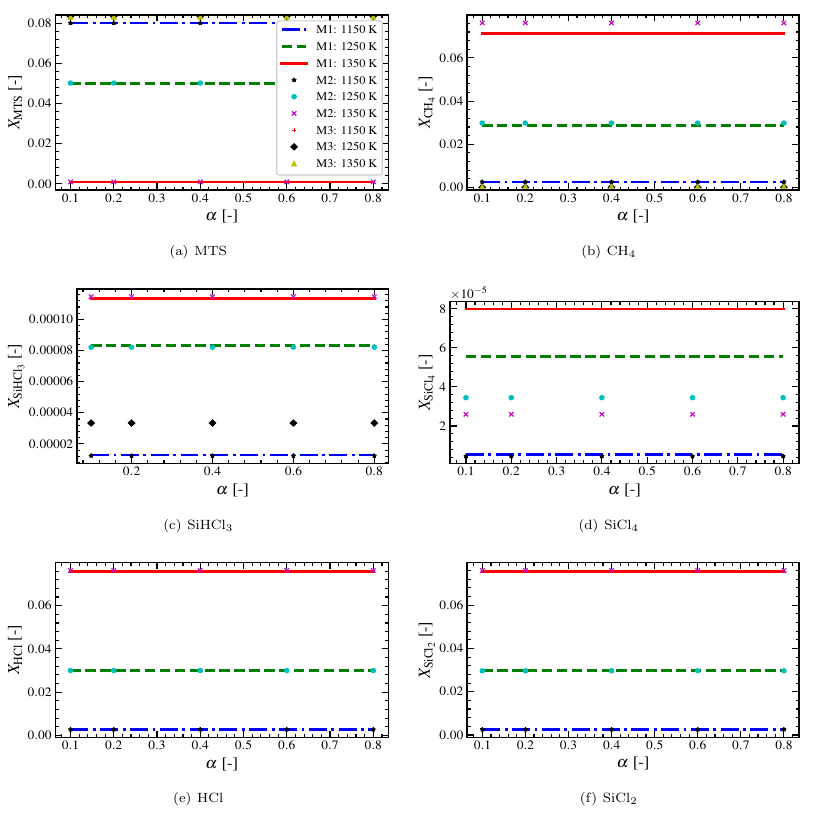
\includegraphics[width=\textwidth]{ph-fig10.png}
    \caption{Variation of mole fraction of MTS (a), CH$_4$ (b), SiHCl$_3$ (c), SiCl$_4$ (d), HCl (e), and SiCl$_2$ (f) with respect to the \% drop in pressure at three values of operating temperature (1150 K, 1250 K, and 1350 K) at inlet pressure of 5 Torr.}
    \label{fig:10}
\end{figure}

Now, we examine the effect of the pressure gradient on the decomposition. To perform this analysis, we consider three inlet pressures, namely, 5 Torr, 52.5 Torr, and 100 Torr. For each inlet pressure, we vary the pressure along the axial direction, leading to a favorable pressure gradient across the reactor, akin to a forced flow condition. We specify the pressure drop, $\Delta P$, across the reactor length $L$ to be $\alpha P$, with the value of $\alpha$ being varied from 10\% to 80\%. This implies that the pressure gradient in the axial direction ($dP/dx$) varies from -7.7 Torr/m to -0.97 Torr/m at $P$ = 5 Torr, from -80.8 Torr/m to -10 Torr/m at $P$ = 52.5 Torr, and from -153.4 Torr/m to 19.2 Torr/m at $P$ = 100 Torr.

Figure \ref{fig:10} shows the effects of $dP/dx$ on the mole fractions of the 6 chemical species at 5 Torr. Overall, we do not observe sensitivity to $dP/dx$ on the variation of any of the considered chemical species. At the inlet pressures of 52.5 Torr and 100 Torr, similar dependence of mole fraction on $dP/dx$ is observed. Therefore, results for these inlet pressures are not included here for the sake of brevity. The major sensitivity is due to the temperature variation. As discussed in Sec. \ref{S:4.2}, the pressure sensitivity was low for the majority of the chemical species, which is also reflected in the lack of sensitivity on the pressure gradient. Even the intermediate reactive species such as SiHCl$_3$ and SiCl$_4$ , which were found to be sensitive to pressure (see Fig. \ref{fig:7}) do not show sensitivity to the considered values of $dP/dx$. These results imply that the MTS decomposition is primarily affected by the reaction mechanism and the kinetics governing the process. 

While MTS, SiHCl$_3$, HCl, and SiCl$_2$ show similar results with the M1 and M2 mechanisms, the results for CH$_4$ and SiCl$_4$ show differences. In particular, the production of CH$_4$ by the M2 mechanism is overpredicted at $T$ = 1350 K. The production of SiCl$_4$ is under-predicted at both 1250 K and 1350 K. These results imply the role of kinetics, which is more sensitive at higher temperatures and availability of the multiple pathways for production/consumption of byproducts and other reactive intermediates in the M1 mechanism.

\subsection{Effects of Compositional Variation}
Now, we examine the effects of compositional variation ($\beta = X_{\rm MTS}/X_{H_2}$) at the inlet by considering $\beta \in (0.05,0.2)$. We consider two types of reactor configurations. In the first case, operating temperature and pressure are specified to be 1250 K and 5 Torr, respectively. In the second case, the pressure is specified to be 5 Torr, however, we consider a temperature gradient of $\Delta T$ = 60 K across the length of the reactor, with the inlet temperature specified to be 1250 K. These conditions are chosen based on the results discussed before, where we observed minor sensitivity to pressure and major sensitivity to temperature and temperature gradient. Figure \ref{fig:11} shows the results from the two types of cases. As the mechanism M3 yields inaccurate results, we only consider M1 and M2 mechanisms to examine the effects of $\beta$.

In the case with temperature gradient, the decomposition of MTS is enhanced, which is apparent from a significant decrease in the value of $X_{\rm MTS}$ for all values of $\beta$. The decrease is much higher for larger values of $\beta$. Such behavior is due to the combined effect of higher temperature and the presence of a temperature gradient. The enhancement in MTS decomposition in the cases with higher temperature gradients is accompanied by an increase in the production of the intermediate reactive species. Furthermore, a higher level of production of these species occurs for larger values of $\beta$. While the variation of mole fraction of species such as SiHCl$_3$, HCl, and SiCl$_2$ with $\beta$ is quasi-linear, the variation of $X_{\rm SiCl_4}$ tends be nonlinear with respect to $\beta$ in both isothermal and temperature gradient cases. Furthermore, the mole fraction of all species from the M2 mechanism matches with the values obtained using the M1 mechanism, which again demonstrates the adequacy of the M2 mechanism for different types of reactor conditions.

The results in this section demonstrate that the decomposition of MTS can be enhanced at a particular operating temperature by enforcing a temperature gradient across the reactor. Such an approach allows for relatively low-temperature conditions to still lead to enhanced decomposition of MTS, which can subsequently assist in SiC deposition on the surface while accounting for the heterogeneous reactions. Note that the commonly used operating temperature for the deposition of SiC matrix composite is around 1200 K to 1300 K. Therefore, with a temperature gradient across the reactor, the decomposition process can be enhanced further.

\section{Conclusions}
\begin{figure}[p]
    \centering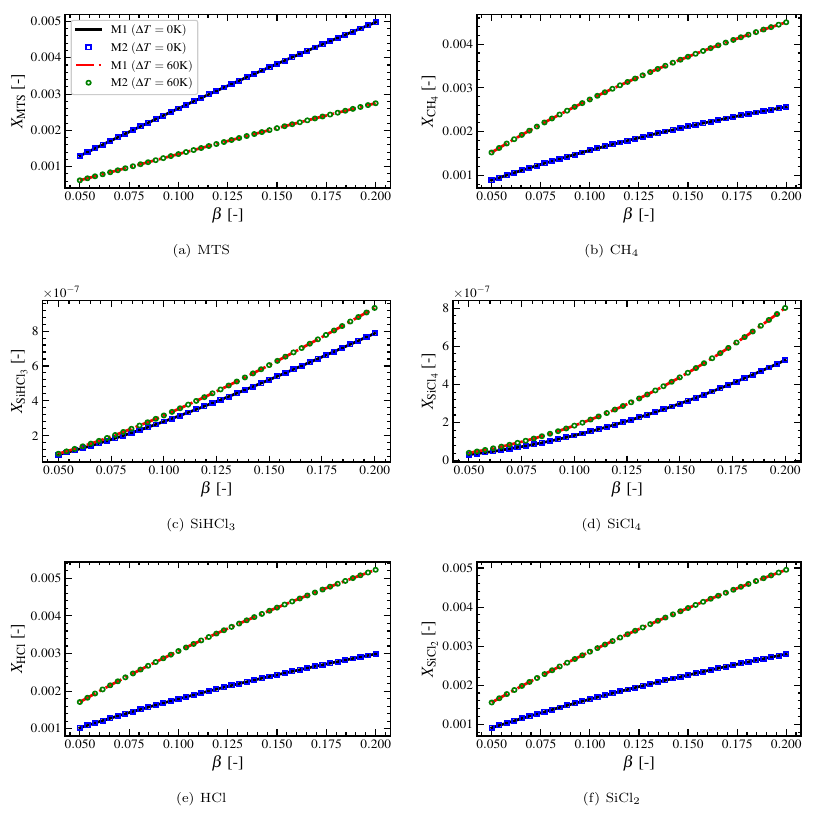
\includegraphics[width=\textwidth]{ph-fig11.png}
    \caption{Variation of mole fraction of MTS (a), CH$_4$ (b), SiHCl$_3$ (c), SiCl$_4$ (d), HCl (e), and SiCl$_2$ (f) with respect to $\beta$ for isothermal and temperature gradient conditions at inlet temperature of 1250 K and pressure of 5 Torr.}
    \label{fig:11}
\end{figure}
CVI is a reliable approach for fabricating high-purity SiC matrix composite, which has excellent thermo- mechanical properties. The quality of the fabricated composite by the CVI process depends upon the employed precursor, gas-phase decomposition, and heterogeneous surface reactions, which in turn are affected by the operating conditions. In this study, a PFR-based computational strategy is utilized to examine the effects of operating conditions on the homogeneous gas-phase decomposition process while using MTS as a precursor with H$_2$ as the carrier gas in a hot-wall cylindrical reactor at CVI-relevant conditions.

The decomposition of MTS leads to the production of several byproducts and intermediate reactive species, which, if not predicted well, can lead to inaccurate results for the subsequent heterogeneous reactions and the associated SiC deposition. Therefore, we considered three chemical mechanisms with varying degree of fidelity, namely, a detailed mechanisms (M1: 103 steps and 42 species), a moderately complex reduced mechanism (M2: 30 steps and 20 species), and a globally reduced mechanism (M3: 1 step and 5 species) to demonstrate that certain number of steps and species are needed to get accurate concentrations of the species. While M1 and M3 mechanisms were considered from past studies, the M2 mechanism was derived from M1 by using a reduction strategy, which ensured that it included the dominant reactions and their sensitivity to key species for the range of operating conditions considered in this study. Compared to the detailed M1 mechanism, the computational cost of a PFR simulation by the M2 and M3 mechanisms was found to be 44.2\% and 26\%, respectively.

The effects of temperature variation were examined for a range of temperatures (1100 K to 1600 K) at three values of pressure (5 Torr, 52.5 Torr, and 100 Torr). The results showed that decomposition of MTS is enhanced beyond 1150 K, and by 1350 K, it was completed. This was accompanied by an increase in the production of CH$_4$ till about 1350 K, followed by a further decomposition of CH$_4$. The byproducts, such as HCl and SiCl$_2$ showed an increased production till 1350 K, followed by a saturation. The other species, such as SiHCl$_3$ and SiCl$_4$ showed a similar behavior where their production showed an increase till about 1350 K, followed by a decrease. These results highlighted the effect of kinetics, which showed significant sensitivity to temperature variations.

The study of the effects of pressure variation was performed for a range of pressures (5 to 100 Torr) at three values of operating temperature (1150 K, 1250 K, and 1350 K). While MTS, CH$_4$, HCl, SiCl$_2$ showed no significant sensitivity to pressure, the species such as SiHCl$_3$, and SiCl$_4$ showed an increase in production with an increase in pressure, where the rate of increase showed an increase with temperature. These results demonstrated the sensitivity of the concentration of various chemical species to the reaction pathways. If the production of a particular species is dependent upon equilibrium-limited reaction or radical recombination, the sensitivity to the pressure is observed. Otherwise, the unimolecular production of species is directly dependent upon MTS decomposition.

The study of the effects of temperature gradient (temperature drop across the reactor) was performed at three inlet temperatures (1150 K, 1250 K, 1350 K) with a temperature gradient of -190 K/m to -19 K/m. The results showed an increased decomposition of MTS due to the presence of a temperature gradient. However, the effect of inlet temperature coupled with the presence of a temperature gradient yielded a complex dependence of the concentration of the species on the specified temperature gradient. The study of the effects of pressure gradient was performed at three values of inlet pressure (5 Torr, 52.5 Torr, and 100 Torr) and inlet temperature (1150 K, 1250 K, and 1350 K) conditions. The results did not show sensitivity to the pressure gradient for the considered conditions, even for some of the reactive intermediate species. These results highlighted the complex interplay of kinetics, thermodynamics, and transport processes, and the presence of multiple pathways for the formation of the reactive intermediate species and byproducts.

Based on the study of effects of operating temperature and pressure conditions on the decomposition of MTS, we identified optimal conditions (1250 K and 5 Torr) and performed the study of effects of compositional variation by varying $\beta$ from 0.05 to 0.2 under isothermal and temperature-gradient scenarios. The variation of mole fraction of species such as SiHCl$_3$, HCl, and SiCl$_2$ with $\beta$ was found to be quasi-linear and the variation of $X_{\rm SiCl_4}$ tend to be nonlinear in both isothermal and temperature-gradient cases. The results also showed that the decomposition of MTS can be enhanced at a particular operating temperature by enforcing a temperature gradient across the reactor.

The results from the moderately complex M2 mechanism showed good agreement with the detailed M1 mechanism under a wide range of operating conditions, thus indicating that it can be used for large-scale simulations under CVI-relevant conditions. The discrepancies observed with the M2 mechanism for some of the species at high temperatures (greater than 1350 K) can be attributed to the absence of about 50\% species in comparison to the M1 mechanism and a significantly lower number of reactions, which affects the thermodynamics and reaction pathways. The study further confirms the limitations of the globally reduced single-step mechanism, such as the M3 mechanism, and emphasizes the need for better reduction approaches.

\section*{Acknowledgements}
This work was supported by the U.S. Department of Energy, Office of Science, Office of Basic Energy Sciences (BES), Gas Phase Chemical Physics (GPCP) through Grant \#DE-SC0024510.

%% References with bibTeX database:
\bibliographystyle{elsarticle-num}
\bibliography{cvi-bib}

\end{document}
